\documentclass[11pt,a4paper]{article}
\usepackage[margin=1in]{geometry}
\usepackage[T1]{fontenc}
\usepackage[utf8]{inputenc}
\usepackage{lmodern}
\usepackage{graphicx}
\usepackage{xurl}
\usepackage{hyperref}
\usepackage{booktabs}
\usepackage{tabularx}
\usepackage{enumitem}
\usepackage{setspace}
\usepackage{caption}
\usepackage{float}

\hypersetup{
  colorlinks=true,
  linkcolor=black,
  urlcolor=blue
}

\graphicspath{
  {assets/}
  {../mfja_robot_control_config/config/room_315_kinematics/debug_plots/}
}

\setstretch{1.03}
\setlist[itemize]{leftmargin=1.2cm}
\setlength{\emergencystretch}{4em}
\sloppy

\title{RECAP Progress Report\\Room 315 Kinematic Shuttle\\Week of April 14--20, 2026}
\author{}
\date{\today}

\begin{document}
\maketitle

\section*{Project Overview}

During this week, the Room 315 shuttle work became a structured kinematic
simulation instead of an early proof of concept. The main idea is simple:
measured CSV rail points provide the geometry, while an explicit rail network
provides the routing logic. The shuttle does not rely on wheel--rail contact
dynamics in this phase. Instead, its pose is computed along the current rail
segment and sent to Gazebo with \texttt{set\_pose}.

This approach made the system easier to test, easier to debug, and much more
stable for demonstrations.

\section*{What Was Completed This Week}

\begin{itemize}
\item Organized the Room 315 rail into 14 directed segments and 12 anchor
nodes.
\item Built \texttt{rail\_network.yaml} with explicit switches, fixed
transitions, stoppers, and start slots.
\item Added CSV preprocessing, network validation, and debug plots.
\item Implemented the kinematic shuttle core with explicit
\texttt{MOVING}, \texttt{WAITING}, and \texttt{FALLING} modes.
\item Added ROS 2 and Gazebo runtime integration for both Room 315 only and the
full-floor world.
\item Added independent switch commands, independent stopper commands, and
sensor-style approach events.
\item Added multi-shuttle support, runtime shuttle spawning, shuttle ON/OFF
control, and start-slot occupancy checks.
\item Added simple collision avoidance with a default distance of
\texttt{0.33 m}.
\item Added a continuous path backend using \texttt{cubic\_hermite}, while
keeping \texttt{polyline} as a reference backend for validation.
\end{itemize}

\section*{Main Problems and How They Were Solved}

\begin{tabularx}{\textwidth}{>{\raggedright\arraybackslash}p{3.3cm} X}
\toprule
\textbf{Problem} & \textbf{Solution} \\
\midrule
Endpoint matching was too fragile & Explicit nodes and routing tables were used
instead of exact endpoint equality. \\
\midrule

Multiple shuttles could overlap & Start-slot occupancy checks and collision
avoidance were added. \\
\midrule

Point-only paths were not the cleanest long-term model & A continuous
\texttt{cubic\_hermite} path backend was introduced and validated against the
CSV polyline reference. \\
\bottomrule
\end{tabularx}

\section*{Current System Picture}

At the end of the week, the system can:

\begin{itemize}
\item launch in Room 315 only or in the full-floor Gazebo world;
\item start one or more shuttles from validated start slots;
\item route shuttles through the rail network according to switch states;
\item stop shuttles before switches with independent stopper commands;
\item publish approach sensor events for teaching and testing;
\item add new shuttles during runtime;
\item enable or disable each shuttle independently;
\item stop following shuttles before they overlap;
\item use continuous path sampling while keeping the CSV files as the measured
source of truth.
\end{itemize}

\section*{Validation Snapshot}

The current network contains:

\begin{itemize}
\item 14 rail segments;
\item 12 nodes;
\item 4 switches;
\item 4 stoppers;
\item 4 validated start slots.
\end{itemize}

The continuous path validator finished with \texttt{PASS} and no warnings. The
maximum deviation between the continuous backend and the polyline reference was
about \texttt{0.00197 m}, which confirms that the new continuous representation
remains very close to the measured path.

\section*{Figures}

\begin{figure}[H]
\centering
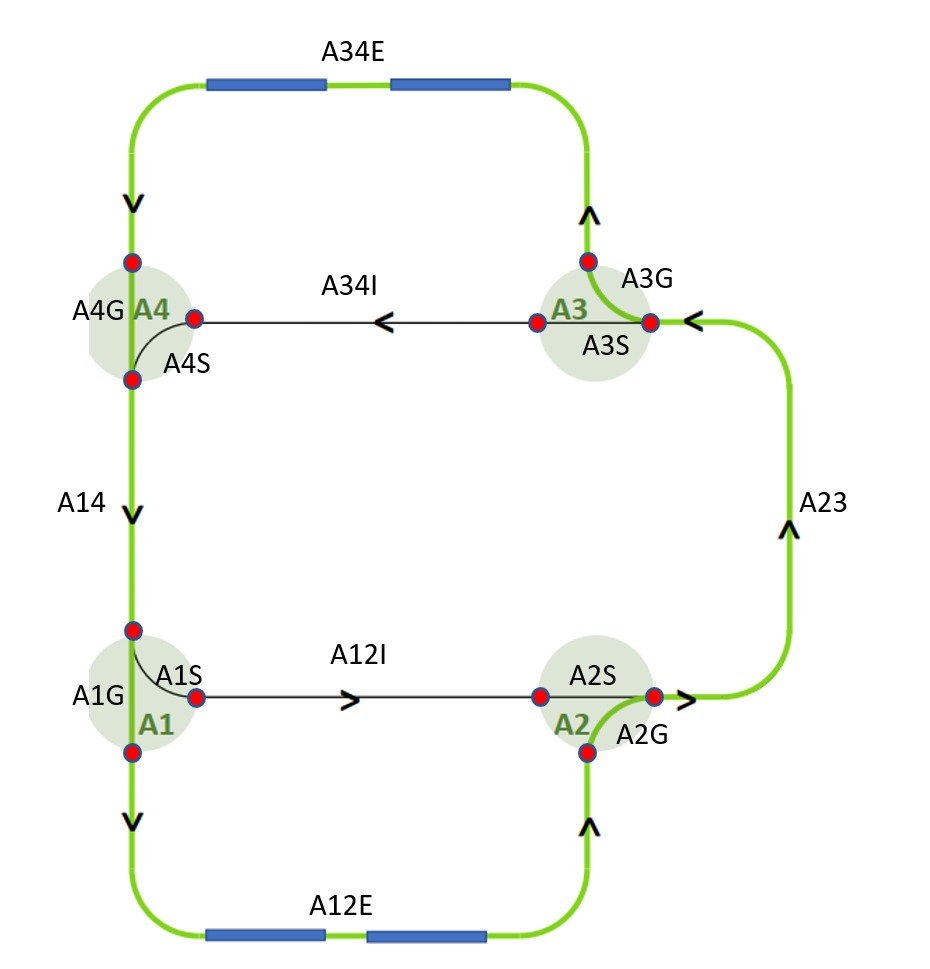
\includegraphics[width=0.86\textwidth]{recqp_topology.jpeg}
\caption{Conceptual Room 315 rail topology used as the basis for the software
network model.}
\end{figure}

\begin{figure}[H]
\centering
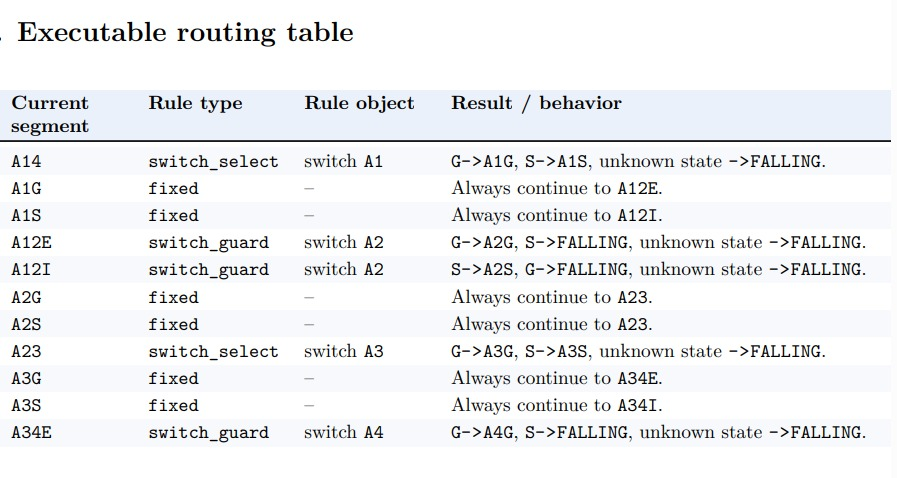
\includegraphics[width=0.96\textwidth]{recqp_routing_table.jpeg}
\caption{Executable routing table idea. Segment transitions are explicit and can
lead to \texttt{FALLING} when the switch configuration is invalid.}
\end{figure}

\begin{figure}[H]
\centering
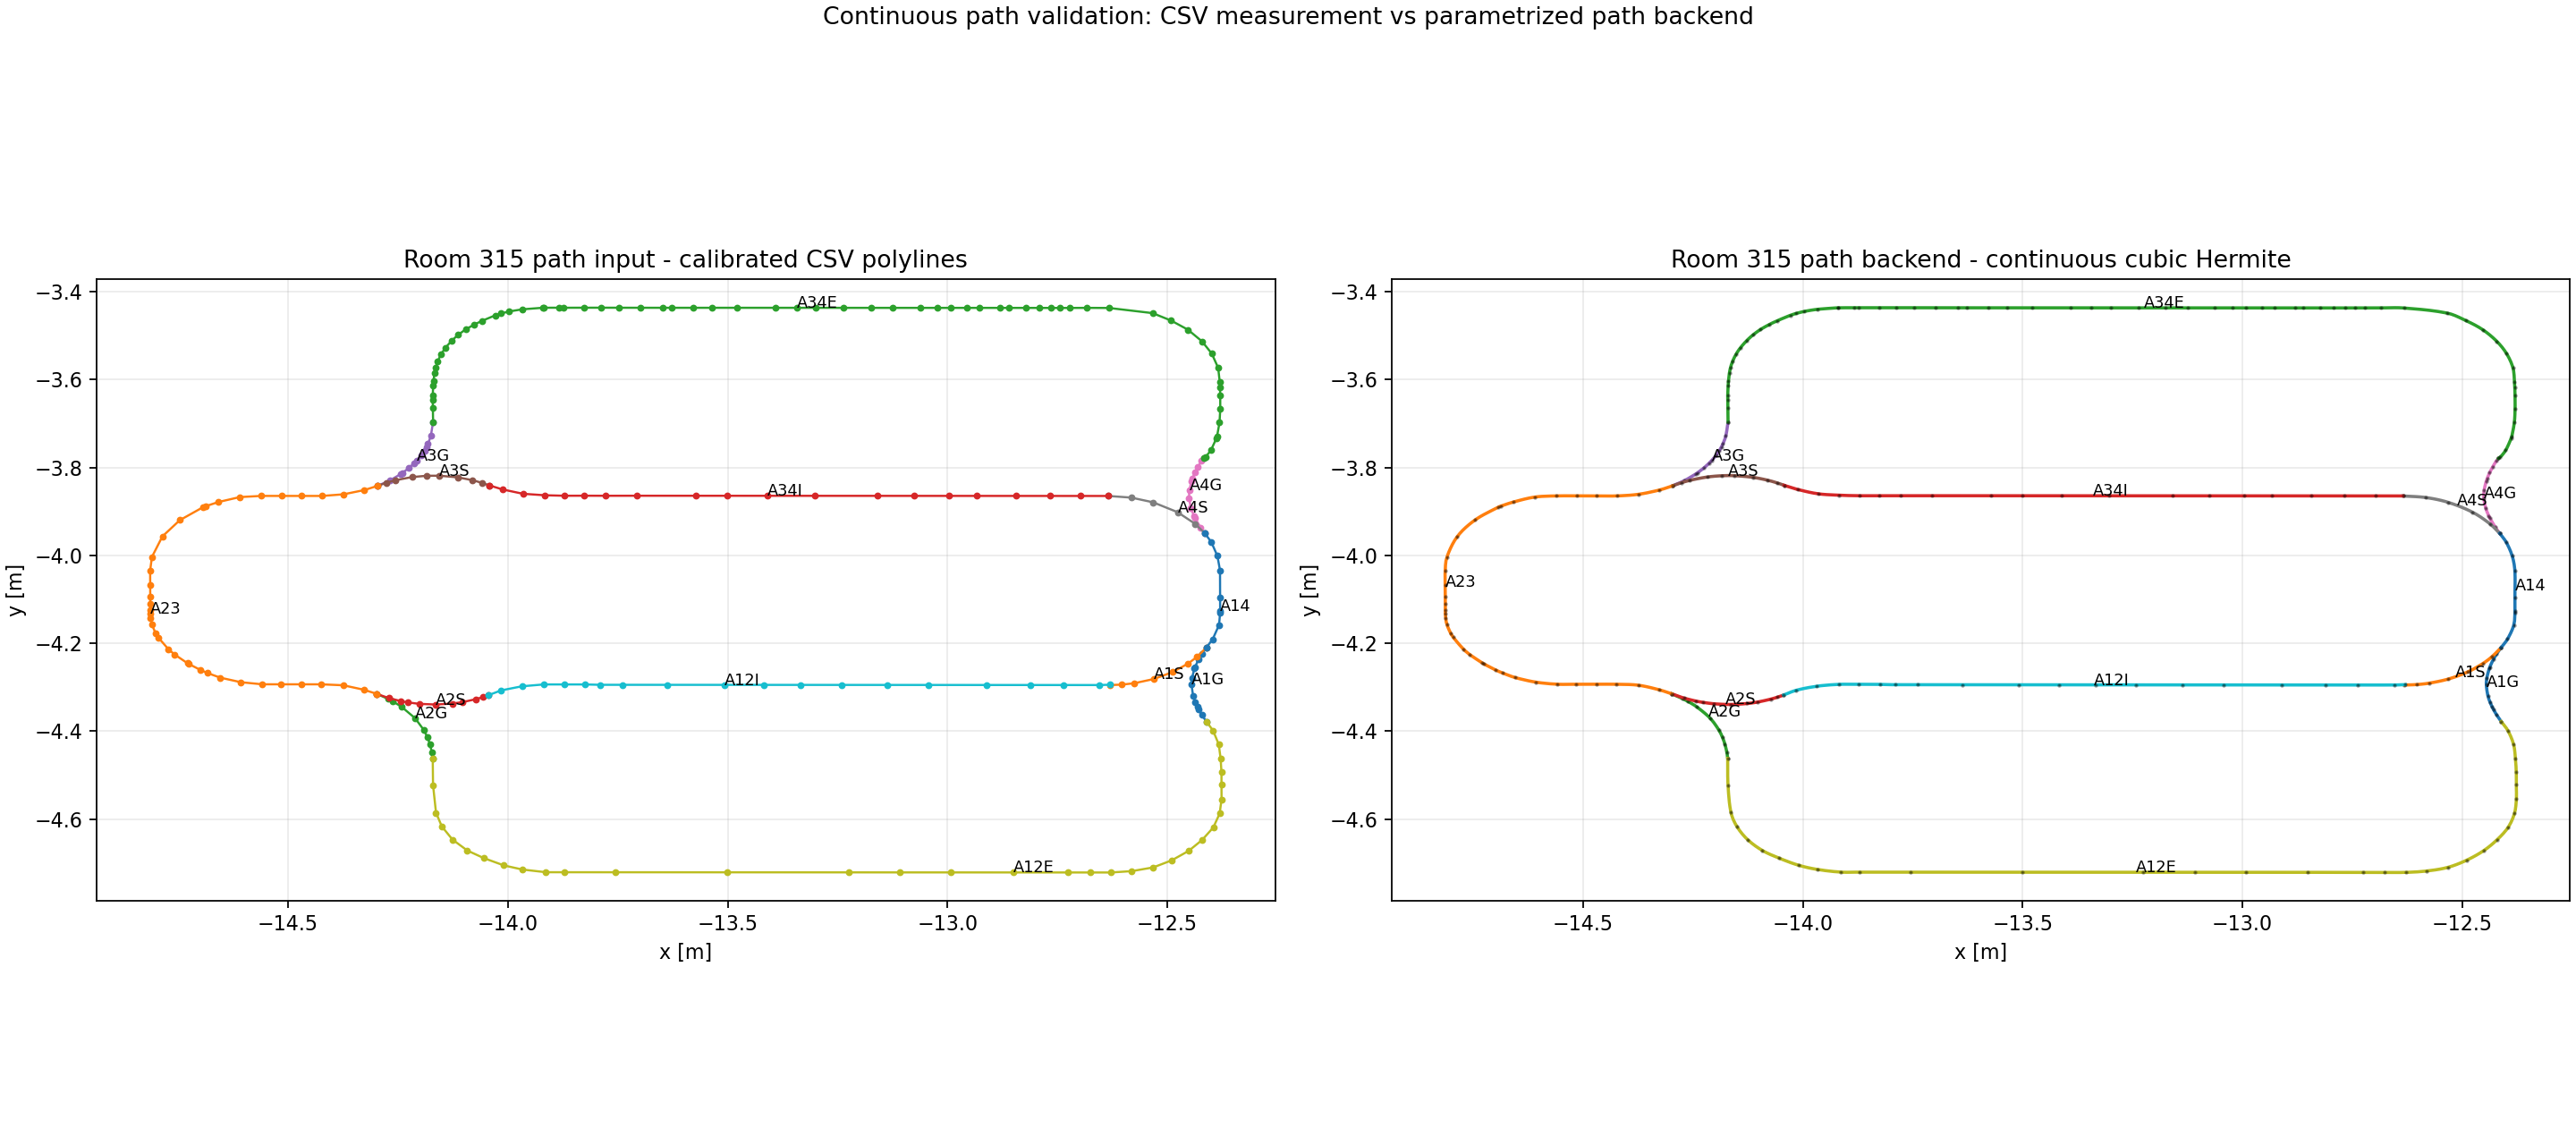
\includegraphics[width=\textwidth]{continuous_path_validation.png}
\caption{Continuous path validation. The \texttt{cubic\_hermite} backend stays
very close to the calibrated CSV polyline while providing smoother runtime
sampling.}
\end{figure}

\section*{Next Step}

\begin{itemize}
\item After finishing one side of the shuttles and sensors, replicate the same
setup on the other side.
\item Adjust the size of the cage.
\item Rename the switch labels to \texttt{exterior} and \texttt{interior}.
\item Make it possible to remove a shuttle completely from the simulation.
\item If shuttles fall, make sure they can be reset without shutting down and
restarting Gazebo.
\end{itemize}

\end{document}
